\documentclass{article}
\usepackage[margin=2.5cm, top=4cm, headheight=25pt]{geometry}
\usepackage{amsmath, amssymb, enumitem, fancyhdr, graphicx}
\usepackage[indent=20pt]{parskip}
\usepackage[hidelinks]{hyperref}
\usepackage{xcolor}
\usepackage{listings}
\usepackage{subcaption}
\usepackage{url}
\usepackage[most]{tcolorbox}
\usepackage{lastpage}

\tcbuselibrary{listingsutf8} % Support for lstlistings within tcolorbox

\newtcolorbox[auto counter, number within=section]{question}[1][]{%
    colframe=gray!80,                      % Dark gray frame
    colback=gray!5,                       % Light gray background
    coltitle=black,                        % Black title
    title=\textbf{Question~\thetcbcounter}, % Bold title
    fonttitle=\bfseries\large,             % Subtle title font size
    rounded corners,                   % Slightly more rounded corners
    boxrule=0.25mm,                         % Thinner border for a sleek look
    enhanced,                              % Enhanced box features
    attach boxed title to top left={xshift=2mm, yshift=-2mm},
    boxed title style={colframe=gray!80, colback=gray!5, boxrule=0.25mm},
    % Title styling
    #1
}

\bibliographystyle{IEEEtran}
\graphicspath{{./images/}}

% -- Custom Variables --
\def\me{Rajdeep Gill 7934493}
\def\course{ECE 3760}
\def\labsection{A01}
\def\labno{1}
\def\title{Log Book}

% -- Styling for code snippets --
\lstset{
    basicstyle=\ttfamily\small,           % Basic font style
    keywordstyle=\color{blue},            % Keywords color
    commentstyle=\color{gray},            % Comments color
    stringstyle=\color{teal},             % Strings color
    numbers=left,                         % Line numbers on the left
    numberstyle=\tiny\color{gray},        % Line number style
    stepnumber=1,                         % Line number step
    numbersep=10pt,                       % Space between line numbers and code
    backgroundcolor=\color{lightgray!10}, % Background color
    frame=single,                         % Adds a frame around the code
    breaklines=true,                      % Line breaking for long lines
    captionpos=b,                         % Caption position
    showspaces=false,                     % Don't show spaces
    showstringspaces=false                % Don't show spaces in strings
}
\renewcommand{\lstlistingname}{Code Snippet}

\renewcommand{\arraystretch}{1.2} % For less-ugly tables
\setlength\parindent{0pt}

%----- Samples 
% Questions:
%   \begin{question}[title=Custom Question Title]
%       Question details
%   \end{question}

% Tables:
%   \begin{table}[htbp]
%       \centering
%       \caption{Table Caption}
%       \begin{tabular}{ll}
%           \toprule
%           \textbf{Column 1} & \textbf{Column 2} \\
%           \midrule
%           Row 1 & Row 2 \\
%           Row 3 & Row 4 \\
%           \bottomrule
%       \end{tabular}
%   \end{table} 

% Figures:
%   Single figure:
%       \begin{figure}[htbp]
%           \centering
%           \includegraphics[width=0.5\textwidth]{example-image}
%           \caption{Figure Caption}
%       \end{figure}
%   Multiple figures:
%       \begin{figure}[htbp]
%           \centering
%           \begin{subfigure}[b]{0.5\textwidth}
%               \includegraphics[width=\textwidth]{example-image-a}
%               \caption{First subfigure}
%           \end{subfigure}
%           \begin{subfigure}[b]{0.5\textwidth}
%               \includegraphics[width=\textwidth]{example-image-b}
%               \caption{Second subfigure}
%           \end{subfigure}
%           \caption{Main figure}
%       \end{figure}

\newcommand{\logbookentry}[2]{
    \subsection*{#1 \hfill \textit{#2}} 
}

\begin{document}

% --------------------------------------------------------------------------------
% TITLE
% --------------------------------------------------------------------------------

\begin{center}
    \huge \title

    \vspace{2mm}
    \hrule

    \vspace{4mm}
    \large \me

    \vspace{2mm}
    \large \course~\labsection

    \vspace{2mm}
    \today
\end{center}

\vspace{4mm}

% --------------------------------------------------------------------------------
% END TITLE
% --------------------------------------------------------------------------------
\vspace{1cm}
\newpage

\pagestyle{fancy}
\fancyhead[L]{\large Logbook}
\fancyhead[R]{\large \me}

\fancyfoot[C]{Page \thepage~of~\pageref{LastPage}}

% --------------------------------------------------------------------------------
% BODY
% --------------------------------------------------------------------------------
\section{Log Entries}

\logbookentry{Lab 1 Entry}{January 20, 2025}
Received the board, soldered pins to the board and ensured that the board was working and no short circuits were present.

Installed platformio on VSCode and ensured the extension was working correctly by running a simple serial print program on the board.

The program was first built and then uploaded to the board, and got a successful message in the console as seen in \autoref{fig:success_upload}.

\begin{figure}[ht!]
    \centering
    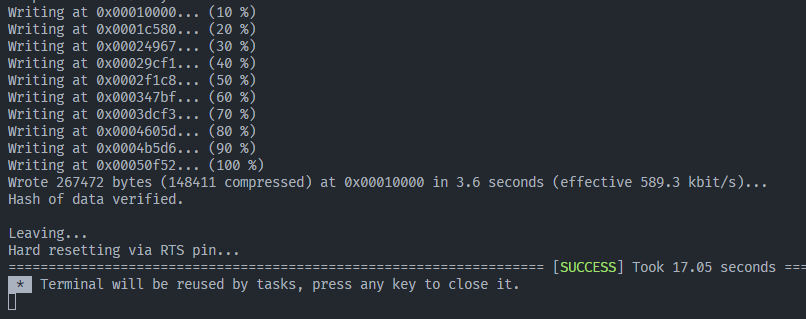
\includegraphics[width=0.8\textwidth]{success_upload.png}
    \caption{Successful upload message in console}
    \label{fig:success_upload}
\end{figure}

\logbookentry{Design Ideas}{January 20, 2025}
During the lab, discussed some ideas for the project. Talked about the basic requirements, what potential ways we can meet the requirements. Need to do more research on how curling actually works to get a better idea of what someone would need to comminicate with their team members to ensure a successful game.

Currently thinking of the skip having a device that can communicate with the two sweepers, having a speed up and slow down button for the sweepers to adjust their speed. The skip would also have a button to indicate when to stop sweeping. On the sweepers side, they would have an LED or a speedometer esque led display to show them how fast they should be sweeping. Since different players might need to sweep at different rates, need to differentiate somehow between the two sweepers. Maybe have two of the same device, but with different colored LEDs or something to indicate which sweeper the skip is talking to. For example, a left and right sweeper device, that connects to the respective sweeper. 

\logbookentry{Individual Design Brainstorming}{January 26, 2025}
A rough sketch of the design I had come up with is provided below. Essentially two sets of controles will be present on the skip's device, one for each sweeper. Along with a display made of LED lights, or other visual indicators to reflect what the sweepers are seeing on there device. 3 buttons will be present, speed up, slow down and an immediate stop button. On the sweeper's device, a line of LED lights or other visual indicators to show a level for the sweeper to sweep at. The skip will be able to adjust the level of the sweeper, and the sweeper will be able to see the level they should be sweeping at.

\begin{figure}[ht!]
    \centering
    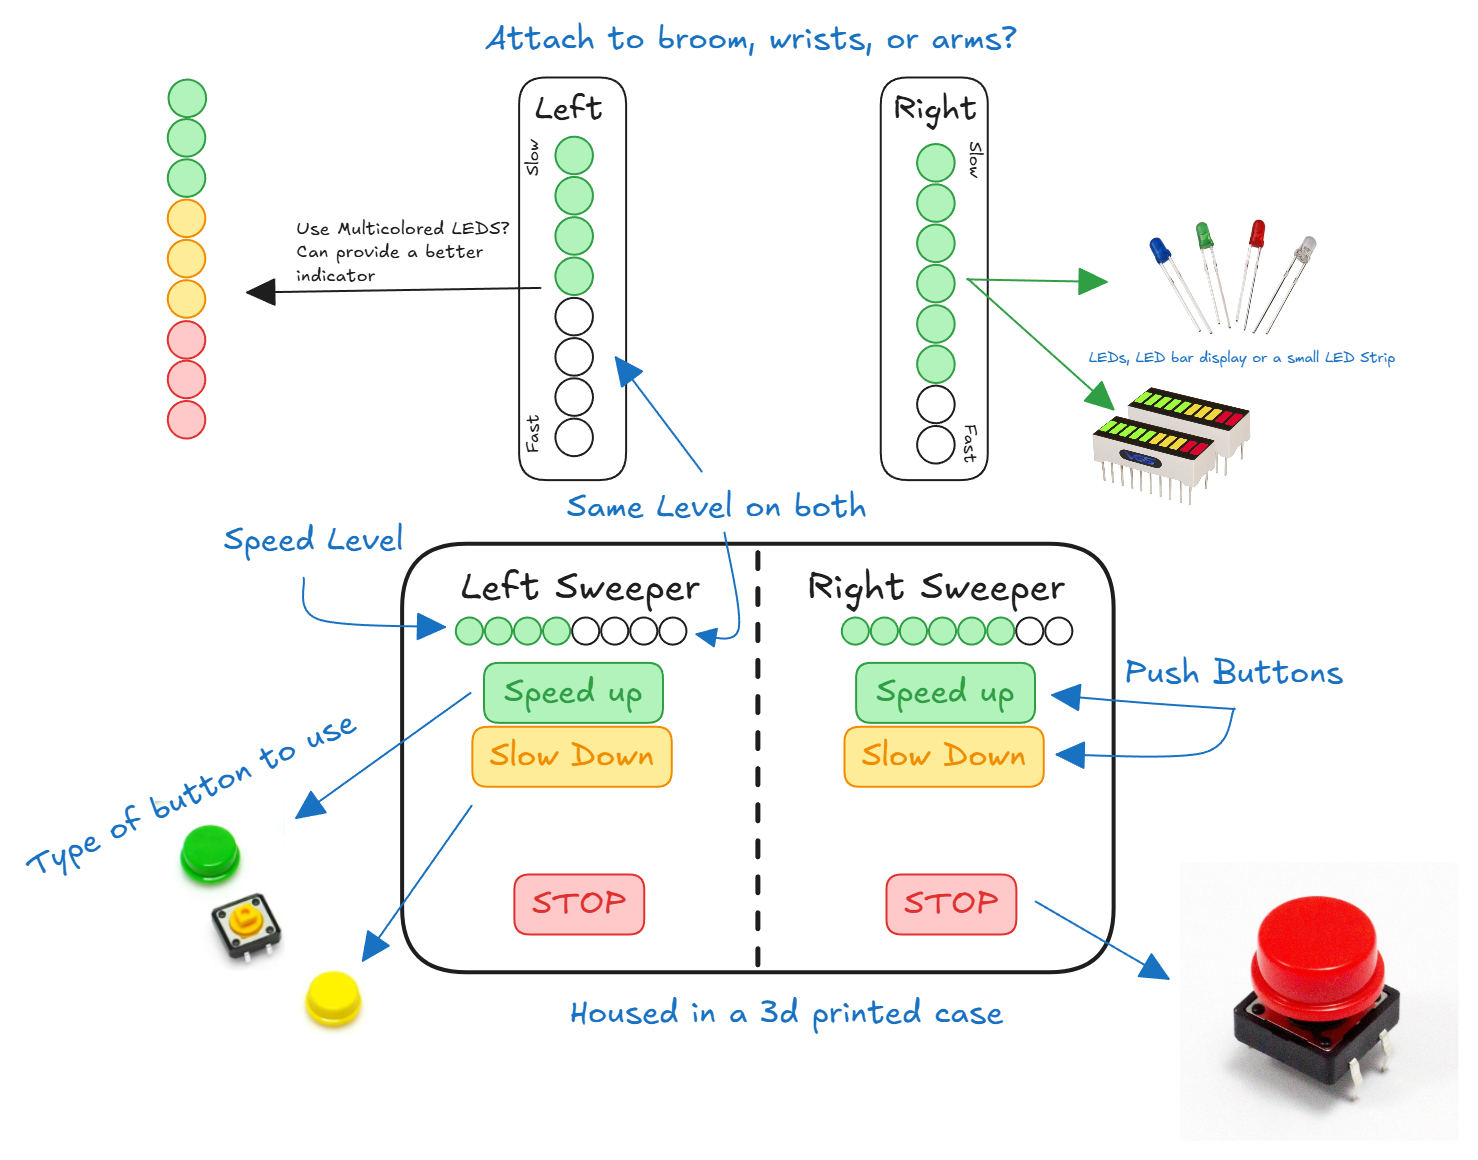
\includegraphics[width=0.7\textwidth]{design_idea1.png}
    \caption{Rough sketch of the design}
\end{figure}
\newpage
The communication between the devices can be done via WiFi as it would have sufficient range to cover the play area. A packet/message structure will need to be defined to ensure the messages are read correctly and by the proper device. A simple message structure could be as follows:

\begin{verbatim}
    <sweeper_id, message_data>
\end{verbatim}
Where \texttt{sweeper\_id} can be a 1 bit for which sweeper, if more than 2 sweepers are present, then we could use 2, 3, 4 bits to represent the sweeper. The message data for each message can be as simple as the level of speed to set the sweeper to, and the sweeper would reply back with an ACK message of the current level they are at to ensure proper synchronization. A simple message-communication diagram is shown below.

\begin{figure}[ht!]
    \centering
    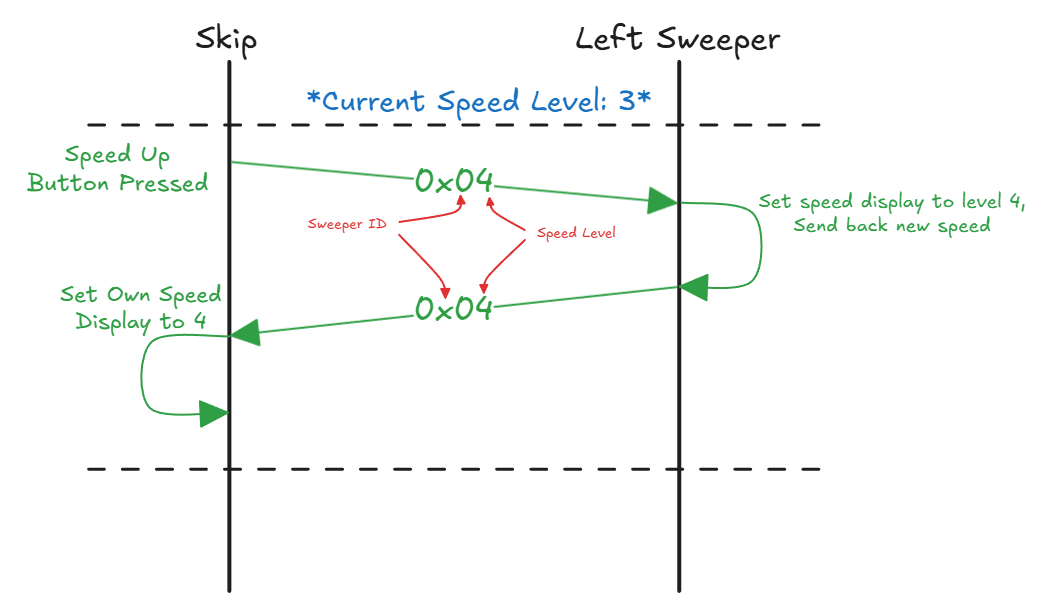
\includegraphics[width=0.6\textwidth]{message_structure_idea.png}
    \caption{Message communication diagram}
\end{figure}

Both sweepers will actively listen to all messages and only act when the \texttt{sweeper\_id} matches their own. This will ensure that the skip can communicate with both sweepers at the same time.

\logbookentry{A Compact Design}{January 28, 2025}
A more compact device for the skip could be used, where a switch can be used to toggle between the two sweepers. This would reduce the size of the device, and essentially reduces the number of components to just half. On the sweepers device a small vibration motor can be used to indicate a message has just arrived. A rough sketch is shown below for the more compact design.
\begin{figure}[ht!]
    \centering
    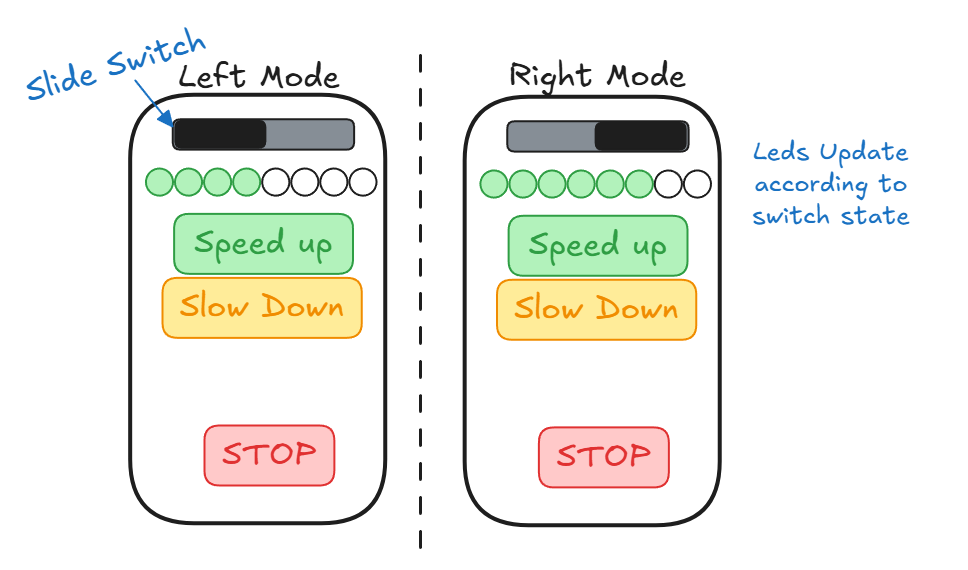
\includegraphics[width=0.8\textwidth]{design_idea2.png}
    \caption{More compact design idea}
\end{figure}

The downside I can see with this is that the skip would need to swap between the two sweepers, which could be a bit cumbersome at times. However, the size reduction could be worth it, and reduced cost of the device. It also will have less LEDs so power consumption could be reduced as well.

\logbookentry{Design Review 1 Reflection}{February 3, 2025}
After the feedback of the initial design review, we have altered our design. Our big oversight was the huge amount of granularity we had in our design. Coming up with multiple sweeping speeds is unecessary and we have learnt that there is really only 3 levels, sweep hard, clean the ice and stop. Outside of this, the curlers will know what to do.

We also have decided to modify our design to contain simpler commands and share the same command to both sweepers. This means that if the skip wants the stone to curl left, we can send the curl left command to both sweepers, and the sweepers will know what to do to make the stone curl left. This will simplify the design and make it easier to implement.

\logbookentry{Lab 2}{February 3, 2025}
The goal of this lab was to get familiar with the ESP32 and the ESP-Now protocol.
We first decoded the positions of a joystick and then controlled LEDs on a ring based on the position of the joystick. The controller was connected to the board at 2 different ADC pins and we read the values of the x and y direction to determine the location. At each position, 8 samples were taken and averaged to get a more resistent value. The x, y values were then used to decode where the joystick was pointing and the LEDs were lit up accordingly.

To light up the LEDs I had used the adafruit neopixel library, allowing me to light any of the 12 LEDs on the ring. The position of the joystick was encoded by a value of 1-9, which represented a position on a grid that was later used to communicate with another device using ESP-Now. The encoding scheme was as follows:
\begin{table}[ht!]
    \centering
    \begin{tabular}{|c|c|c|}
        \hline
        NW & N & NE \\
        9 & 8 & 7 \\
        \hline 
        W & C & E \\
        6 & 5 & 4 \\
        \hline
        SW & S & SE \\
        3 & 2 & 1 \\
        \hline
    \end{tabular}
    \caption{Joystick encoding scheme}
\end{table}

A function was created which took a direction value, 1 through 9, and lit up the corresponding LED(s).

In the last part of the lab, we had obtained the mac address of a differnet device to communicate via ESP-Now. We established a connection between the sender and receiver and then send a message containing the encoded joystick position to the receiver. The receiver would then light up the corresponding LED on the ring. The communication was successful and the LEDs lit up as expected. There was a short delay added as to not overload the network with messages.

\textbf{Questions for Lab 2}
\begin{enumerate}
    \item The joystick was powered by the 3.3V and grounded by the GND pin. Two ADC1 pins were used to read the x and y values of the joystick. For the LED ring, the data pin was connected to a GPIO pin on the ESP32, and powered in a similar fashion to the joystick.
    \item The folow of the program is as follows:
    \begin{itemize}
        \item Connect with receiver via ESP-Now
        \item Initialize the LED ring
        \item Main Loop:
        \item Sample x and y values 8 times and average them
        \item Decode the position of the joystick into one of 9 positions
        \item Send the position to the receiver via ESP-Now
        \item Receive the position and light up the corresponding LED
    \end{itemize}

    \item To improve the usability of the device, a difference decoding scheme from the coordinates to position could be used. Currently there exists some deadzones where the joystick is close to one position but LEDs do not light up.

    \item There were no major performance issues, aside from the added delay as to not overload the network. The LEDs lit up as expected and the joystick was able to control the LEDs. Doing a serial print, it was able to detect and decode the position in a very fast manner.
    \item Technical questions:
    \begin{enumerate}[label=\alph*.]
        \item The transmitter needs to know the MAC address of the receiver because ESP-NOW does not use IP addresses like regular Wi-Fi. Instead, devices communicate directly using their unique MAC addresses. This helps the sender know exactly which device to send data to. Without the MAC address, the transmitter wouldn`'t know where to send the message. There is an option to broadcast the message to all devices by using the mac address of 0xFF.

        \item We are not able to determine if the message was received, only if it was sent succesfully. To ensure the message was received, we could implement a handshake protocol where the receiver sends an ACK message back to the transmitter. This would ensure that the message was received and understood by the receiver.
        \item \begin{enumerate}
            \item There is no way to authenticate that the packet was specifically meant for a target device if it is broadcasted. However, we can add extra details in the packet to ensure that the receiver knows that the packet was meant for them. This could be a simple ID, or a more complex encryption scheme to ensure that the packet was meant for the receiver.
            \item The transmitter would not know if the message was received by the target device by default. However, as discussed above, we can implement a handshake protocol.
            \item As more devices transmit on the network, we would have more congestion and sending messages could take longer and even fail if the network is too congested. This is why we had added an artifical delay to ensure that the network was not overloaded with messages.
        \end{enumerate}
    \end{enumerate}
\end{enumerate}

\logbookentry{Design Refinement}{February 5, 2025}
The new design idea contains a more simplified setup. 5 buttons are present on the skips device along with an LED ring. The sweepers device will be a simple case with the same LED ring. The commands will be sent to both sweepers at the same time. We will also show the command for a brief period before turning the LEDs off, which will allow for better power consumption. The different commands will light up different parts of the LEDs in various colors to make it as easy as possible for the sweepers to differentiate the different commands. The current command encoding for the LEDs is as follows. This is preliminary and could change as we test the design. The goal would be to make it as easy as possible for the sweepers to understand the command.
\begin{table}[ht!]
    \centering
    \begin{tabular}{|c|c|}
        \hline 
        \textbf{Command} & \textbf{LEDs} \\
        \hline
        Sweep Hard & Green - Fully lit \\
        Clean Ice & Blue - Top Half \\
        Stop & Red - Fully lit \\
        Curl Left & Blue - Left Half \\
        Curl Right & Blue - Right Half \\
        \hline
    \end{tabular}
    \caption{Encoding for LEDs}
\end{table}

\logbookentry{PCB Assignment}{February 9, 2025}
The PCB assignment was done succesfully without any errors. Initially I had picked the EasyEDA pro option, but then switched to the std edition as it was easier and more intuitive to use. The artistic element included on the PCB was a meme of a guy pointing towards the required information on the back of the board.

The design of the PCB is from class, a Human-Machine-Interface board with push buttons, an analog input and a screen. We utilize an OLED screen, 2 push buttons, a potentiometer and a status LED. The screen is controlled by an I$^2$C interface, the push buttons are connected to two seperate pins, and the potentiometer is connected to a different pin. A generic 8-pin header is also present to connect to a MCU to control the board.

\logbookentry{PCB Assignment - Bill of Materials}{February 11, 2025}
The bill of materials with sources for the PCB we designed as follows:
\begin{table}[ht!]
    \centering
    \begin{tabular}{|c|c|c|c|c|}
        \hline
        \textbf{Part} & \textbf{Quantity} & \textbf{Price} & \textbf{Total} & \textbf{Source} \\
        \hline
        Capacitor & 3 & \$0.03442  & \$0.10326 
        &\href{https://www.digikey.ca/en/products/detail/kemet/C0805C104K3RACTU/411167}{\underline{DigiKey}} \\
        Header Pin & 1 & \$0.11134 & \$0.11134 & \href{https://www.digikey.ca/en/products/detail/adam-tech/PH1-08-UA/9830442}{\underline{DigiKey}} \\
        Push Button & 2 & \$0.62256 & \$1.24512 & \href{https://www.digikey.ca/en/products/detail/schurter-inc/1301-9314-24/8536705}{\underline{DigiKey}}\\
        LED & 1 & \$0.18192 & \$0.18192 & \href{https://www.digikey.ca/en/products/detail/w%C3%BCrth-elektronik/150060BS55040/8557178}{\underline{DigiKey}} \\
        Resistors & 5 & \$0.00619 & \$0.03095 & \href{https://www.digikey.ca/en/products/detail/bourns-inc/CR0603-JW-102ELF/3741004}{\underline{DigiKey}} \\
        Potentiometer & 1 & \$1.40968 & \$1.40968 & \href{https://www.digikey.ca/en/products/detail/bourns-inc/3386P-1-202LF/1088527}{\underline{DigiKey}} \\
        OLED Screen & 1 & \$11.99  & \$11.99 & \href{https://www.waveshare.com/1.54inch-oled-module.htm}{\underline{Waveshare}} \\
        \hline
        \multicolumn{3}{|r|}{\textbf{Total}} & \$15.07 & - \\
        \hline
    \end{tabular}
    \caption{Bill of Materials}
\end{table}

The OLED screen was sourced from waveshare and is of the same specification as the one used in the PCB. It is a 1.54 inch OLED screen with a resolution of 128x64 pixels with an I$^2$C interface. Other parts were sourced from DigiKey, and were picked to fit the footprint on the PCB and the requirements of the board.


 






% --------------------------------------------------------------------------------
% END BODY
% --------------------------------------------------------------------------------

\end{document}
